\documentclass{standalone}
\usepackage{xcolor}
\usepackage{tikz}
\usetikzlibrary{positioning, shapes.multipart, calc, graphs, graphs.standard, arrows.meta}
\begin{document}
\begin{tikzpicture}[x=15.0pt, y=15.0pt, scale=2.0]
% style: major_grid
\tikzstyle{major_grid}=[black,step=20pt]
% style: minor_grid
\tikzstyle{minor_grid}=[very thin,step=10pt]
% style: defaultEdge
\tikzstyle{defaultEdge}=[thick,out=-90,in=90,out distance=1.5cm,in distance=1.5cm,looseness=1.5]
% style: defaultLabel
\tikzstyle{defaultLabel}=[auto,anchor=south west]
% style: OperationLayer_style
\tikzstyle{OperationLayer_style}=[rectangle split,rectangle split ignore empty parts,very thick,rectangle split parts=5,draw=violet!80,fill=violet!5,minimum width=4cm,outer sep=0cm,inner sep=2pt]
% style: UtilityLayer_style
\tikzstyle{UtilityLayer_style}=[rectangle split,rectangle split ignore empty parts,very thick,rectangle split parts=5,draw=gray!80,fill=gray!5,minimum width=4cm,outer sep=0cm,inner sep=2pt]
% style: TrainableLayer_style
\tikzstyle{TrainableLayer_style}=[rectangle split,rectangle split ignore empty parts,very thick,rectangle split parts=5,draw=blue!80,fill=blue!5,minimum width=4cm,outer sep=0cm,inner sep=2pt]

% node group: input_1_group
% node: input_1
\node[TrainableLayer_style] (input_1) at (20.0, 400.0)
    {
    \nodepart{one}{InputLayer}
    \nodepart{two}{input shape: (224, 224, 3)}};
% end of node group: input_1_group

% node group: Conv1_group
% node: bn_Conv1
\node[UtilityLayer_style] (bn_Conv1) at (20.0, 395.05)
    {
    \nodepart{one}{BatchNormalization}};
% node: Conv1
\node[TrainableLayer_style] (Conv1) at (20.0, 396.12)
    {
    \nodepart{one}{Conv2D}
    \nodepart{two}{filters: 32}
    \nodepart{three}{kernel: (3, 3)}
    \nodepart{four}{activation: linear}};
% end of node group: Conv1_group

% node group: Conv1_relu_group
% node: Conv1_relu
\node[TrainableLayer_style] (Conv1_relu) at (20.0, 392.23)
    {
    \nodepart{one}{ReLU}};
% end of node group: Conv1_relu_group

% node group: expanded_conv_depthwise_group
% node: expanded_conv_depthwise_BN
\node[UtilityLayer_style] (expanded_conv_depthwise_BN) at (20.0, 387.28)
    {
    \nodepart{one}{BatchNormalization}};
% node: expanded_conv_depthwise
\node[TrainableLayer_style] (expanded_conv_depthwise) at (20.0, 388.35)
    {
    \nodepart{one}{DepthwiseConv2D}
    \nodepart{two}{kernel: (3, 3)}
    \nodepart{three}{depth multiplier: 1}
    \nodepart{four}{activation: linear}};
% end of node group: expanded_conv_depthwise_group

% node group: expanded_conv_depthwise_relu_group
% node: expanded_conv_depthwise_relu
\node[TrainableLayer_style] (expanded_conv_depthwise_relu) at (20.0, 384.47)
    {
    \nodepart{one}{ReLU}};
% end of node group: expanded_conv_depthwise_relu_group

% node group: expanded_conv_project_group
% node: expanded_conv_project_BN
\node[UtilityLayer_style] (expanded_conv_project_BN) at (20.0, 379.51)
    {
    \nodepart{one}{BatchNormalization}};
% node: expanded_conv_project
\node[TrainableLayer_style] (expanded_conv_project) at (20.0, 380.58)
    {
    \nodepart{one}{Conv2D}
    \nodepart{two}{filters: 16}
    \nodepart{three}{kernel: (1, 1)}
    \nodepart{four}{activation: linear}};
% end of node group: expanded_conv_project_group

% node group: block_1_expand_group
% node: block_1_expand_BN
\node[UtilityLayer_style] (block_1_expand_BN) at (20.0, 375.63)
    {
    \nodepart{one}{BatchNormalization}};
% node: block_1_expand
\node[TrainableLayer_style] (block_1_expand) at (20.0, 376.7)
    {
    \nodepart{one}{Conv2D}
    \nodepart{two}{filters: 96}
    \nodepart{three}{kernel: (1, 1)}
    \nodepart{four}{activation: linear}};
% end of node group: block_1_expand_group

% node group: block_1_expand_relu_group
% node: block_1_expand_relu
\node[TrainableLayer_style] (block_1_expand_relu) at (20.0, 372.82)
    {
    \nodepart{one}{ReLU}};
% end of node group: block_1_expand_relu_group

% node group: block_1_pad_group
% node: block_1_pad
\node[TrainableLayer_style] (block_1_pad) at (20.0, 368.93)
    {
    \nodepart{one}{ZeroPadding2D}
    \nodepart{two}{padding: ((0, 1), (0, 1))}};
% end of node group: block_1_pad_group

% node group: block_1_depthwise_group
% node: block_1_depthwise_BN
\node[UtilityLayer_style] (block_1_depthwise_BN) at (20.0, 363.98)
    {
    \nodepart{one}{BatchNormalization}};
% node: block_1_depthwise
\node[TrainableLayer_style] (block_1_depthwise) at (20.0, 365.05)
    {
    \nodepart{one}{DepthwiseConv2D}
    \nodepart{two}{kernel: (3, 3)}
    \nodepart{three}{depth multiplier: 1}
    \nodepart{four}{activation: linear}};
% end of node group: block_1_depthwise_group

% node group: block_1_depthwise_relu_group
% node: block_1_depthwise_relu
\node[TrainableLayer_style] (block_1_depthwise_relu) at (20.0, 361.17)
    {
    \nodepart{one}{ReLU}};
% end of node group: block_1_depthwise_relu_group

% node group: block_1_project_group
% node: block_1_project_BN
\node[UtilityLayer_style] (block_1_project_BN) at (20.0, 356.21)
    {
    \nodepart{one}{BatchNormalization}};
% node: block_1_project
\node[TrainableLayer_style] (block_1_project) at (20.0, 357.28)
    {
    \nodepart{one}{Conv2D}
    \nodepart{two}{filters: 24}
    \nodepart{three}{kernel: (1, 1)}
    \nodepart{four}{activation: linear}};
% end of node group: block_1_project_group

% node group: block_2_expand_group
% node: block_2_expand_BN
\node[UtilityLayer_style] (block_2_expand_BN) at (0.0, 352.33)
    {
    \nodepart{one}{BatchNormalization}};
% node: block_2_expand
\node[TrainableLayer_style] (block_2_expand) at (0.0, 353.4)
    {
    \nodepart{one}{Conv2D}
    \nodepart{two}{filters: 144}
    \nodepart{three}{kernel: (1, 1)}
    \nodepart{four}{activation: linear}};
% end of node group: block_2_expand_group

% node group: block_2_add_group
% node: block_2_add
\node[OperationLayer_style] (block_2_add) at (20.0, 333.98)
    {
    \nodepart{one}{Add}};
% end of node group: block_2_add_group

% node group: block_3_expand_group
% node: block_3_expand_BN
\node[UtilityLayer_style] (block_3_expand_BN) at (20.0, 329.03)
    {
    \nodepart{one}{BatchNormalization}};
% node: block_3_expand
\node[TrainableLayer_style] (block_3_expand) at (20.0, 330.1)
    {
    \nodepart{one}{Conv2D}
    \nodepart{two}{filters: 144}
    \nodepart{three}{kernel: (1, 1)}
    \nodepart{four}{activation: linear}};
% end of node group: block_3_expand_group

% node group: block_2_expand_relu_group
% node: block_2_expand_relu
\node[TrainableLayer_style] (block_2_expand_relu) at (0.0, 349.51)
    {
    \nodepart{one}{ReLU}};
% end of node group: block_2_expand_relu_group

% node group: block_2_depthwise_group
% node: block_2_depthwise_BN
\node[UtilityLayer_style] (block_2_depthwise_BN) at (0.0, 344.56)
    {
    \nodepart{one}{BatchNormalization}};
% node: block_2_depthwise
\node[TrainableLayer_style] (block_2_depthwise) at (0.0, 345.63)
    {
    \nodepart{one}{DepthwiseConv2D}
    \nodepart{two}{kernel: (3, 3)}
    \nodepart{three}{depth multiplier: 1}
    \nodepart{four}{activation: linear}};
% end of node group: block_2_depthwise_group

% node group: block_3_expand_relu_group
% node: block_3_expand_relu
\node[TrainableLayer_style] (block_3_expand_relu) at (20.0, 326.21)
    {
    \nodepart{one}{ReLU}};
% end of node group: block_3_expand_relu_group

% node group: block_3_pad_group
% node: block_3_pad
\node[TrainableLayer_style] (block_3_pad) at (20.0, 322.33)
    {
    \nodepart{one}{ZeroPadding2D}
    \nodepart{two}{padding: ((0, 1), (0, 1))}};
% end of node group: block_3_pad_group

% node group: block_2_depthwise_relu_group
% node: block_2_depthwise_relu
\node[TrainableLayer_style] (block_2_depthwise_relu) at (0.0, 341.75)
    {
    \nodepart{one}{ReLU}};
% end of node group: block_2_depthwise_relu_group

% node group: block_3_depthwise_group
% node: block_3_depthwise_BN
\node[UtilityLayer_style] (block_3_depthwise_BN) at (20.0, 317.38)
    {
    \nodepart{one}{BatchNormalization}};
% node: block_3_depthwise
\node[TrainableLayer_style] (block_3_depthwise) at (20.0, 318.45)
    {
    \nodepart{one}{DepthwiseConv2D}
    \nodepart{two}{kernel: (3, 3)}
    \nodepart{three}{depth multiplier: 1}
    \nodepart{four}{activation: linear}};
% end of node group: block_3_depthwise_group

% node group: block_2_project_group
% node: block_2_project_BN
\node[UtilityLayer_style] (block_2_project_BN) at (0.0, 336.79)
    {
    \nodepart{one}{BatchNormalization}};
% node: block_2_project
\node[TrainableLayer_style] (block_2_project) at (0.0, 337.86)
    {
    \nodepart{one}{Conv2D}
    \nodepart{two}{filters: 24}
    \nodepart{three}{kernel: (1, 1)}
    \nodepart{four}{activation: linear}};
% end of node group: block_2_project_group

% node group: block_3_depthwise_relu_group
% node: block_3_depthwise_relu
\node[TrainableLayer_style] (block_3_depthwise_relu) at (20.0, 314.56)
    {
    \nodepart{one}{ReLU}};
% end of node group: block_3_depthwise_relu_group

% node group: block_3_project_group
% node: block_3_project_BN
\node[UtilityLayer_style] (block_3_project_BN) at (20.0, 309.61)
    {
    \nodepart{one}{BatchNormalization}};
% node: block_3_project
\node[TrainableLayer_style] (block_3_project) at (20.0, 310.68)
    {
    \nodepart{one}{Conv2D}
    \nodepart{two}{filters: 32}
    \nodepart{three}{kernel: (1, 1)}
    \nodepart{four}{activation: linear}};
% end of node group: block_3_project_group

% node group: block_4_expand_group
% node: block_4_expand_BN
\node[UtilityLayer_style] (block_4_expand_BN) at (0.0, 305.73)
    {
    \nodepart{one}{BatchNormalization}};
% node: block_4_expand
\node[TrainableLayer_style] (block_4_expand) at (0.0, 306.8)
    {
    \nodepart{one}{Conv2D}
    \nodepart{two}{filters: 192}
    \nodepart{three}{kernel: (1, 1)}
    \nodepart{four}{activation: linear}};
% end of node group: block_4_expand_group

% node group: block_4_add_group
% node: block_4_add
\node[OperationLayer_style] (block_4_add) at (20.0, 287.38)
    {
    \nodepart{one}{Add}};
% end of node group: block_4_add_group

% node group: block_5_expand_group
% node: block_5_expand_BN
\node[UtilityLayer_style] (block_5_expand_BN) at (0.0, 282.43)
    {
    \nodepart{one}{BatchNormalization}};
% node: block_5_expand
\node[TrainableLayer_style] (block_5_expand) at (0.0, 283.5)
    {
    \nodepart{one}{Conv2D}
    \nodepart{two}{filters: 192}
    \nodepart{three}{kernel: (1, 1)}
    \nodepart{four}{activation: linear}};
% end of node group: block_5_expand_group

% node group: block_5_add_group
% node: block_5_add
\node[OperationLayer_style] (block_5_add) at (20.0, 264.08)
    {
    \nodepart{one}{Add}};
% end of node group: block_5_add_group

% node group: block_4_expand_relu_group
% node: block_4_expand_relu
\node[TrainableLayer_style] (block_4_expand_relu) at (0.0, 302.91)
    {
    \nodepart{one}{ReLU}};
% end of node group: block_4_expand_relu_group

% node group: block_6_expand_group
% node: block_6_expand_BN
\node[UtilityLayer_style] (block_6_expand_BN) at (20.0, 259.12)
    {
    \nodepart{one}{BatchNormalization}};
% node: block_6_expand
\node[TrainableLayer_style] (block_6_expand) at (20.0, 260.19)
    {
    \nodepart{one}{Conv2D}
    \nodepart{two}{filters: 192}
    \nodepart{three}{kernel: (1, 1)}
    \nodepart{four}{activation: linear}};
% end of node group: block_6_expand_group

% node group: block_4_depthwise_group
% node: block_4_depthwise_BN
\node[UtilityLayer_style] (block_4_depthwise_BN) at (0.0, 297.96)
    {
    \nodepart{one}{BatchNormalization}};
% node: block_4_depthwise
\node[TrainableLayer_style] (block_4_depthwise) at (0.0, 299.03)
    {
    \nodepart{one}{DepthwiseConv2D}
    \nodepart{two}{kernel: (3, 3)}
    \nodepart{three}{depth multiplier: 1}
    \nodepart{four}{activation: linear}};
% end of node group: block_4_depthwise_group

% node group: block_5_expand_relu_group
% node: block_5_expand_relu
\node[TrainableLayer_style] (block_5_expand_relu) at (0.0, 279.61)
    {
    \nodepart{one}{ReLU}};
% end of node group: block_5_expand_relu_group

% node group: block_5_depthwise_group
% node: block_5_depthwise_BN
\node[UtilityLayer_style] (block_5_depthwise_BN) at (0.0, 274.66)
    {
    \nodepart{one}{BatchNormalization}};
% node: block_5_depthwise
\node[TrainableLayer_style] (block_5_depthwise) at (0.0, 275.73)
    {
    \nodepart{one}{DepthwiseConv2D}
    \nodepart{two}{kernel: (3, 3)}
    \nodepart{three}{depth multiplier: 1}
    \nodepart{four}{activation: linear}};
% end of node group: block_5_depthwise_group

% node group: block_6_expand_relu_group
% node: block_6_expand_relu
\node[TrainableLayer_style] (block_6_expand_relu) at (20.0, 256.31)
    {
    \nodepart{one}{ReLU}};
% end of node group: block_6_expand_relu_group

% node group: block_4_depthwise_relu_group
% node: block_4_depthwise_relu
\node[TrainableLayer_style] (block_4_depthwise_relu) at (0.0, 295.15)
    {
    \nodepart{one}{ReLU}};
% end of node group: block_4_depthwise_relu_group

% node group: block_6_pad_group
% node: block_6_pad
\node[TrainableLayer_style] (block_6_pad) at (20.0, 252.43)
    {
    \nodepart{one}{ZeroPadding2D}
    \nodepart{two}{padding: ((0, 1), (0, 1))}};
% end of node group: block_6_pad_group

% node group: block_4_project_group
% node: block_4_project_BN
\node[UtilityLayer_style] (block_4_project_BN) at (0.0, 290.19)
    {
    \nodepart{one}{BatchNormalization}};
% node: block_4_project
\node[TrainableLayer_style] (block_4_project) at (0.0, 291.26)
    {
    \nodepart{one}{Conv2D}
    \nodepart{two}{filters: 32}
    \nodepart{three}{kernel: (1, 1)}
    \nodepart{four}{activation: linear}};
% end of node group: block_4_project_group

% node group: block_5_depthwise_relu_group
% node: block_5_depthwise_relu
\node[TrainableLayer_style] (block_5_depthwise_relu) at (0.0, 271.84)
    {
    \nodepart{one}{ReLU}};
% end of node group: block_5_depthwise_relu_group

% node group: block_6_depthwise_group
% node: block_6_depthwise_BN
\node[UtilityLayer_style] (block_6_depthwise_BN) at (20.0, 247.47)
    {
    \nodepart{one}{BatchNormalization}};
% node: block_6_depthwise
\node[TrainableLayer_style] (block_6_depthwise) at (20.0, 248.54)
    {
    \nodepart{one}{DepthwiseConv2D}
    \nodepart{two}{kernel: (3, 3)}
    \nodepart{three}{depth multiplier: 1}
    \nodepart{four}{activation: linear}};
% end of node group: block_6_depthwise_group

% node group: block_5_project_group
% node: block_5_project_BN
\node[UtilityLayer_style] (block_5_project_BN) at (0.0, 266.89)
    {
    \nodepart{one}{BatchNormalization}};
% node: block_5_project
\node[TrainableLayer_style] (block_5_project) at (0.0, 267.96)
    {
    \nodepart{one}{Conv2D}
    \nodepart{two}{filters: 32}
    \nodepart{three}{kernel: (1, 1)}
    \nodepart{four}{activation: linear}};
% end of node group: block_5_project_group

% node group: block_6_depthwise_relu_group
% node: block_6_depthwise_relu
\node[TrainableLayer_style] (block_6_depthwise_relu) at (20.0, 244.66)
    {
    \nodepart{one}{ReLU}};
% end of node group: block_6_depthwise_relu_group

% node group: block_6_project_group
% node: block_6_project_BN
\node[UtilityLayer_style] (block_6_project_BN) at (20.0, 239.71)
    {
    \nodepart{one}{BatchNormalization}};
% node: block_6_project
\node[TrainableLayer_style] (block_6_project) at (20.0, 240.78)
    {
    \nodepart{one}{Conv2D}
    \nodepart{two}{filters: 64}
    \nodepart{three}{kernel: (1, 1)}
    \nodepart{four}{activation: linear}};
% end of node group: block_6_project_group

% node group: block_7_expand_group
% node: block_7_expand_BN
\node[UtilityLayer_style] (block_7_expand_BN) at (0.0, 235.82)
    {
    \nodepart{one}{BatchNormalization}};
% node: block_7_expand
\node[TrainableLayer_style] (block_7_expand) at (0.0, 236.89)
    {
    \nodepart{one}{Conv2D}
    \nodepart{two}{filters: 384}
    \nodepart{three}{kernel: (1, 1)}
    \nodepart{four}{activation: linear}};
% end of node group: block_7_expand_group

% node group: block_7_add_group
% node: block_7_add
\node[OperationLayer_style] (block_7_add) at (20.0, 217.48)
    {
    \nodepart{one}{Add}};
% end of node group: block_7_add_group

% node group: block_8_expand_group
% node: block_8_expand_BN
\node[UtilityLayer_style] (block_8_expand_BN) at (0.0, 212.52)
    {
    \nodepart{one}{BatchNormalization}};
% node: block_8_expand
\node[TrainableLayer_style] (block_8_expand) at (0.0, 213.59)
    {
    \nodepart{one}{Conv2D}
    \nodepart{two}{filters: 384}
    \nodepart{three}{kernel: (1, 1)}
    \nodepart{four}{activation: linear}};
% end of node group: block_8_expand_group

% node group: block_8_add_group
% node: block_8_add
\node[OperationLayer_style] (block_8_add) at (20.0, 194.17)
    {
    \nodepart{one}{Add}};
% end of node group: block_8_add_group

% node group: block_7_expand_relu_group
% node: block_7_expand_relu
\node[TrainableLayer_style] (block_7_expand_relu) at (0.0, 233.01)
    {
    \nodepart{one}{ReLU}};
% end of node group: block_7_expand_relu_group

% node group: block_9_expand_group
% node: block_9_expand_BN
\node[UtilityLayer_style] (block_9_expand_BN) at (0.0, 189.22)
    {
    \nodepart{one}{BatchNormalization}};
% node: block_9_expand
\node[TrainableLayer_style] (block_9_expand) at (0.0, 190.29)
    {
    \nodepart{one}{Conv2D}
    \nodepart{two}{filters: 384}
    \nodepart{three}{kernel: (1, 1)}
    \nodepart{four}{activation: linear}};
% end of node group: block_9_expand_group

% node group: block_9_add_group
% node: block_9_add
\node[OperationLayer_style] (block_9_add) at (20.0, 170.87)
    {
    \nodepart{one}{Add}};
% end of node group: block_9_add_group

% node group: block_7_depthwise_group
% node: block_7_depthwise_BN
\node[UtilityLayer_style] (block_7_depthwise_BN) at (0.0, 228.06)
    {
    \nodepart{one}{BatchNormalization}};
% node: block_7_depthwise
\node[TrainableLayer_style] (block_7_depthwise) at (0.0, 229.13)
    {
    \nodepart{one}{DepthwiseConv2D}
    \nodepart{two}{kernel: (3, 3)}
    \nodepart{three}{depth multiplier: 1}
    \nodepart{four}{activation: linear}};
% end of node group: block_7_depthwise_group

% node group: block_8_expand_relu_group
% node: block_8_expand_relu
\node[TrainableLayer_style] (block_8_expand_relu) at (0.0, 209.71)
    {
    \nodepart{one}{ReLU}};
% end of node group: block_8_expand_relu_group

% node group: block_10_expand_group
% node: block_10_expand_BN
\node[UtilityLayer_style] (block_10_expand_BN) at (20.0, 165.92)
    {
    \nodepart{one}{BatchNormalization}};
% node: block_10_expand
\node[TrainableLayer_style] (block_10_expand) at (20.0, 166.99)
    {
    \nodepart{one}{Conv2D}
    \nodepart{two}{filters: 384}
    \nodepart{three}{kernel: (1, 1)}
    \nodepart{four}{activation: linear}};
% end of node group: block_10_expand_group

% node group: block_8_depthwise_group
% node: block_8_depthwise_BN
\node[UtilityLayer_style] (block_8_depthwise_BN) at (0.0, 204.76)
    {
    \nodepart{one}{BatchNormalization}};
% node: block_8_depthwise
\node[TrainableLayer_style] (block_8_depthwise) at (0.0, 205.83)
    {
    \nodepart{one}{DepthwiseConv2D}
    \nodepart{two}{kernel: (3, 3)}
    \nodepart{three}{depth multiplier: 1}
    \nodepart{four}{activation: linear}};
% end of node group: block_8_depthwise_group

% node group: block_9_expand_relu_group
% node: block_9_expand_relu
\node[TrainableLayer_style] (block_9_expand_relu) at (0.0, 186.41)
    {
    \nodepart{one}{ReLU}};
% end of node group: block_9_expand_relu_group

% node group: block_7_depthwise_relu_group
% node: block_7_depthwise_relu
\node[TrainableLayer_style] (block_7_depthwise_relu) at (0.0, 225.24)
    {
    \nodepart{one}{ReLU}};
% end of node group: block_7_depthwise_relu_group

% node group: block_9_depthwise_group
% node: block_9_depthwise_BN
\node[UtilityLayer_style] (block_9_depthwise_BN) at (0.0, 181.45)
    {
    \nodepart{one}{BatchNormalization}};
% node: block_9_depthwise
\node[TrainableLayer_style] (block_9_depthwise) at (0.0, 182.52)
    {
    \nodepart{one}{DepthwiseConv2D}
    \nodepart{two}{kernel: (3, 3)}
    \nodepart{three}{depth multiplier: 1}
    \nodepart{four}{activation: linear}};
% end of node group: block_9_depthwise_group

% node group: block_10_expand_relu_group
% node: block_10_expand_relu
\node[TrainableLayer_style] (block_10_expand_relu) at (20.0, 163.11)
    {
    \nodepart{one}{ReLU}};
% end of node group: block_10_expand_relu_group

% node group: block_7_project_group
% node: block_7_project_BN
\node[UtilityLayer_style] (block_7_project_BN) at (0.0, 220.29)
    {
    \nodepart{one}{BatchNormalization}};
% node: block_7_project
\node[TrainableLayer_style] (block_7_project) at (0.0, 221.36)
    {
    \nodepart{one}{Conv2D}
    \nodepart{two}{filters: 64}
    \nodepart{three}{kernel: (1, 1)}
    \nodepart{four}{activation: linear}};
% end of node group: block_7_project_group

% node group: block_8_depthwise_relu_group
% node: block_8_depthwise_relu
\node[TrainableLayer_style] (block_8_depthwise_relu) at (0.0, 201.94)
    {
    \nodepart{one}{ReLU}};
% end of node group: block_8_depthwise_relu_group

% node group: block_10_depthwise_group
% node: block_10_depthwise_BN
\node[UtilityLayer_style] (block_10_depthwise_BN) at (20.0, 158.15)
    {
    \nodepart{one}{BatchNormalization}};
% node: block_10_depthwise
\node[TrainableLayer_style] (block_10_depthwise) at (20.0, 159.22)
    {
    \nodepart{one}{DepthwiseConv2D}
    \nodepart{two}{kernel: (3, 3)}
    \nodepart{three}{depth multiplier: 1}
    \nodepart{four}{activation: linear}};
% end of node group: block_10_depthwise_group

% node group: block_8_project_group
% node: block_8_project_BN
\node[UtilityLayer_style] (block_8_project_BN) at (0.0, 196.99)
    {
    \nodepart{one}{BatchNormalization}};
% node: block_8_project
\node[TrainableLayer_style] (block_8_project) at (0.0, 198.06)
    {
    \nodepart{one}{Conv2D}
    \nodepart{two}{filters: 64}
    \nodepart{three}{kernel: (1, 1)}
    \nodepart{four}{activation: linear}};
% end of node group: block_8_project_group

% node group: block_9_depthwise_relu_group
% node: block_9_depthwise_relu
\node[TrainableLayer_style] (block_9_depthwise_relu) at (0.0, 178.64)
    {
    \nodepart{one}{ReLU}};
% end of node group: block_9_depthwise_relu_group

% node group: block_9_project_group
% node: block_9_project_BN
\node[UtilityLayer_style] (block_9_project_BN) at (0.0, 173.69)
    {
    \nodepart{one}{BatchNormalization}};
% node: block_9_project
\node[TrainableLayer_style] (block_9_project) at (0.0, 174.76)
    {
    \nodepart{one}{Conv2D}
    \nodepart{two}{filters: 64}
    \nodepart{three}{kernel: (1, 1)}
    \nodepart{four}{activation: linear}};
% end of node group: block_9_project_group

% node group: block_10_depthwise_relu_group
% node: block_10_depthwise_relu
\node[TrainableLayer_style] (block_10_depthwise_relu) at (20.0, 155.34)
    {
    \nodepart{one}{ReLU}};
% end of node group: block_10_depthwise_relu_group

% node group: block_10_project_group
% node: block_10_project_BN
\node[UtilityLayer_style] (block_10_project_BN) at (20.0, 150.39)
    {
    \nodepart{one}{BatchNormalization}};
% node: block_10_project
\node[TrainableLayer_style] (block_10_project) at (20.0, 151.46)
    {
    \nodepart{one}{Conv2D}
    \nodepart{two}{filters: 96}
    \nodepart{three}{kernel: (1, 1)}
    \nodepart{four}{activation: linear}};
% end of node group: block_10_project_group

% node group: block_11_expand_group
% node: block_11_expand_BN
\node[UtilityLayer_style] (block_11_expand_BN) at (0.0, 146.5)
    {
    \nodepart{one}{BatchNormalization}};
% node: block_11_expand
\node[TrainableLayer_style] (block_11_expand) at (0.0, 147.57)
    {
    \nodepart{one}{Conv2D}
    \nodepart{two}{filters: 576}
    \nodepart{three}{kernel: (1, 1)}
    \nodepart{four}{activation: linear}};
% end of node group: block_11_expand_group

% node group: block_11_add_group
% node: block_11_add
\node[OperationLayer_style] (block_11_add) at (20.0, 128.16)
    {
    \nodepart{one}{Add}};
% end of node group: block_11_add_group

% node group: block_12_expand_group
% node: block_12_expand_BN
\node[UtilityLayer_style] (block_12_expand_BN) at (0.0, 123.2)
    {
    \nodepart{one}{BatchNormalization}};
% node: block_12_expand
\node[TrainableLayer_style] (block_12_expand) at (0.0, 124.27)
    {
    \nodepart{one}{Conv2D}
    \nodepart{two}{filters: 576}
    \nodepart{three}{kernel: (1, 1)}
    \nodepart{four}{activation: linear}};
% end of node group: block_12_expand_group

% node group: block_12_add_group
% node: block_12_add
\node[OperationLayer_style] (block_12_add) at (20.0, 104.85)
    {
    \nodepart{one}{Add}};
% end of node group: block_12_add_group

% node group: block_11_expand_relu_group
% node: block_11_expand_relu
\node[TrainableLayer_style] (block_11_expand_relu) at (0.0, 143.69)
    {
    \nodepart{one}{ReLU}};
% end of node group: block_11_expand_relu_group

% node group: block_13_expand_group
% node: block_13_expand_BN
\node[UtilityLayer_style] (block_13_expand_BN) at (20.0, 99.9)
    {
    \nodepart{one}{BatchNormalization}};
% node: block_13_expand
\node[TrainableLayer_style] (block_13_expand) at (20.0, 100.97)
    {
    \nodepart{one}{Conv2D}
    \nodepart{two}{filters: 576}
    \nodepart{three}{kernel: (1, 1)}
    \nodepart{four}{activation: linear}};
% end of node group: block_13_expand_group

% node group: block_11_depthwise_group
% node: block_11_depthwise_BN
\node[UtilityLayer_style] (block_11_depthwise_BN) at (0.0, 138.74)
    {
    \nodepart{one}{BatchNormalization}};
% node: block_11_depthwise
\node[TrainableLayer_style] (block_11_depthwise) at (0.0, 139.81)
    {
    \nodepart{one}{DepthwiseConv2D}
    \nodepart{two}{kernel: (3, 3)}
    \nodepart{three}{depth multiplier: 1}
    \nodepart{four}{activation: linear}};
% end of node group: block_11_depthwise_group

% node group: block_12_expand_relu_group
% node: block_12_expand_relu
\node[TrainableLayer_style] (block_12_expand_relu) at (0.0, 120.39)
    {
    \nodepart{one}{ReLU}};
% end of node group: block_12_expand_relu_group

% node group: block_12_depthwise_group
% node: block_12_depthwise_BN
\node[UtilityLayer_style] (block_12_depthwise_BN) at (0.0, 115.43)
    {
    \nodepart{one}{BatchNormalization}};
% node: block_12_depthwise
\node[TrainableLayer_style] (block_12_depthwise) at (0.0, 116.5)
    {
    \nodepart{one}{DepthwiseConv2D}
    \nodepart{two}{kernel: (3, 3)}
    \nodepart{three}{depth multiplier: 1}
    \nodepart{four}{activation: linear}};
% end of node group: block_12_depthwise_group

% node group: block_13_expand_relu_group
% node: block_13_expand_relu
\node[TrainableLayer_style] (block_13_expand_relu) at (20.0, 97.09)
    {
    \nodepart{one}{ReLU}};
% end of node group: block_13_expand_relu_group

% node group: block_11_depthwise_relu_group
% node: block_11_depthwise_relu
\node[TrainableLayer_style] (block_11_depthwise_relu) at (0.0, 135.92)
    {
    \nodepart{one}{ReLU}};
% end of node group: block_11_depthwise_relu_group

% node group: block_13_pad_group
% node: block_13_pad
\node[TrainableLayer_style] (block_13_pad) at (20.0, 93.2)
    {
    \nodepart{one}{ZeroPadding2D}
    \nodepart{two}{padding: ((0, 1), (0, 1))}};
% end of node group: block_13_pad_group

% node group: block_11_project_group
% node: block_11_project_BN
\node[UtilityLayer_style] (block_11_project_BN) at (0.0, 130.97)
    {
    \nodepart{one}{BatchNormalization}};
% node: block_11_project
\node[TrainableLayer_style] (block_11_project) at (0.0, 132.04)
    {
    \nodepart{one}{Conv2D}
    \nodepart{two}{filters: 96}
    \nodepart{three}{kernel: (1, 1)}
    \nodepart{four}{activation: linear}};
% end of node group: block_11_project_group

% node group: block_12_depthwise_relu_group
% node: block_12_depthwise_relu
\node[TrainableLayer_style] (block_12_depthwise_relu) at (0.0, 112.62)
    {
    \nodepart{one}{ReLU}};
% end of node group: block_12_depthwise_relu_group

% node group: block_13_depthwise_group
% node: block_13_depthwise_BN
\node[UtilityLayer_style] (block_13_depthwise_BN) at (20.0, 88.25)
    {
    \nodepart{one}{BatchNormalization}};
% node: block_13_depthwise
\node[TrainableLayer_style] (block_13_depthwise) at (20.0, 89.32)
    {
    \nodepart{one}{DepthwiseConv2D}
    \nodepart{two}{kernel: (3, 3)}
    \nodepart{three}{depth multiplier: 1}
    \nodepart{four}{activation: linear}};
% end of node group: block_13_depthwise_group

% node group: block_12_project_group
% node: block_12_project_BN
\node[UtilityLayer_style] (block_12_project_BN) at (0.0, 107.67)
    {
    \nodepart{one}{BatchNormalization}};
% node: block_12_project
\node[TrainableLayer_style] (block_12_project) at (0.0, 108.74)
    {
    \nodepart{one}{Conv2D}
    \nodepart{two}{filters: 96}
    \nodepart{three}{kernel: (1, 1)}
    \nodepart{four}{activation: linear}};
% end of node group: block_12_project_group

% node group: block_13_depthwise_relu_group
% node: block_13_depthwise_relu
\node[TrainableLayer_style] (block_13_depthwise_relu) at (20.0, 85.44)
    {
    \nodepart{one}{ReLU}};
% end of node group: block_13_depthwise_relu_group

% node group: block_13_project_group
% node: block_13_project_BN
\node[UtilityLayer_style] (block_13_project_BN) at (20.0, 80.48)
    {
    \nodepart{one}{BatchNormalization}};
% node: block_13_project
\node[TrainableLayer_style] (block_13_project) at (20.0, 81.55)
    {
    \nodepart{one}{Conv2D}
    \nodepart{two}{filters: 160}
    \nodepart{three}{kernel: (1, 1)}
    \nodepart{four}{activation: linear}};
% end of node group: block_13_project_group

% node group: block_14_expand_group
% node: block_14_expand_BN
\node[UtilityLayer_style] (block_14_expand_BN) at (0.0, 76.6)
    {
    \nodepart{one}{BatchNormalization}};
% node: block_14_expand
\node[TrainableLayer_style] (block_14_expand) at (0.0, 77.67)
    {
    \nodepart{one}{Conv2D}
    \nodepart{two}{filters: 960}
    \nodepart{three}{kernel: (1, 1)}
    \nodepart{four}{activation: linear}};
% end of node group: block_14_expand_group

% node group: block_14_add_group
% node: block_14_add
\node[OperationLayer_style] (block_14_add) at (20.0, 58.25)
    {
    \nodepart{one}{Add}};
% end of node group: block_14_add_group

% node group: block_15_expand_group
% node: block_15_expand_BN
\node[UtilityLayer_style] (block_15_expand_BN) at (0.0, 53.3)
    {
    \nodepart{one}{BatchNormalization}};
% node: block_15_expand
\node[TrainableLayer_style] (block_15_expand) at (0.0, 54.37)
    {
    \nodepart{one}{Conv2D}
    \nodepart{two}{filters: 960}
    \nodepart{three}{kernel: (1, 1)}
    \nodepart{four}{activation: linear}};
% end of node group: block_15_expand_group

% node group: block_15_add_group
% node: block_15_add
\node[OperationLayer_style] (block_15_add) at (20.0, 34.95)
    {
    \nodepart{one}{Add}};
% end of node group: block_15_add_group

% node group: block_14_expand_relu_group
% node: block_14_expand_relu
\node[TrainableLayer_style] (block_14_expand_relu) at (0.0, 73.79)
    {
    \nodepart{one}{ReLU}};
% end of node group: block_14_expand_relu_group

% node group: block_16_expand_group
% node: block_16_expand_BN
\node[UtilityLayer_style] (block_16_expand_BN) at (20.0, 30.0)
    {
    \nodepart{one}{BatchNormalization}};
% node: block_16_expand
\node[TrainableLayer_style] (block_16_expand) at (20.0, 31.07)
    {
    \nodepart{one}{Conv2D}
    \nodepart{two}{filters: 960}
    \nodepart{three}{kernel: (1, 1)}
    \nodepart{four}{activation: linear}};
% end of node group: block_16_expand_group

% node group: block_14_depthwise_group
% node: block_14_depthwise_BN
\node[UtilityLayer_style] (block_14_depthwise_BN) at (0.0, 68.83)
    {
    \nodepart{one}{BatchNormalization}};
% node: block_14_depthwise
\node[TrainableLayer_style] (block_14_depthwise) at (0.0, 69.9)
    {
    \nodepart{one}{DepthwiseConv2D}
    \nodepart{two}{kernel: (3, 3)}
    \nodepart{three}{depth multiplier: 1}
    \nodepart{four}{activation: linear}};
% end of node group: block_14_depthwise_group

% node group: block_15_expand_relu_group
% node: block_15_expand_relu
\node[TrainableLayer_style] (block_15_expand_relu) at (0.0, 50.49)
    {
    \nodepart{one}{ReLU}};
% end of node group: block_15_expand_relu_group

% node group: block_15_depthwise_group
% node: block_15_depthwise_BN
\node[UtilityLayer_style] (block_15_depthwise_BN) at (0.0, 45.53)
    {
    \nodepart{one}{BatchNormalization}};
% node: block_15_depthwise
\node[TrainableLayer_style] (block_15_depthwise) at (0.0, 46.6)
    {
    \nodepart{one}{DepthwiseConv2D}
    \nodepart{two}{kernel: (3, 3)}
    \nodepart{three}{depth multiplier: 1}
    \nodepart{four}{activation: linear}};
% end of node group: block_15_depthwise_group

% node group: block_16_expand_relu_group
% node: block_16_expand_relu
\node[TrainableLayer_style] (block_16_expand_relu) at (20.0, 27.18)
    {
    \nodepart{one}{ReLU}};
% end of node group: block_16_expand_relu_group

% node group: block_14_depthwise_relu_group
% node: block_14_depthwise_relu
\node[TrainableLayer_style] (block_14_depthwise_relu) at (0.0, 66.02)
    {
    \nodepart{one}{ReLU}};
% end of node group: block_14_depthwise_relu_group

% node group: block_16_depthwise_group
% node: block_16_depthwise_BN
\node[UtilityLayer_style] (block_16_depthwise_BN) at (20.0, 22.23)
    {
    \nodepart{one}{BatchNormalization}};
% node: block_16_depthwise
\node[TrainableLayer_style] (block_16_depthwise) at (20.0, 23.3)
    {
    \nodepart{one}{DepthwiseConv2D}
    \nodepart{two}{kernel: (3, 3)}
    \nodepart{three}{depth multiplier: 1}
    \nodepart{four}{activation: linear}};
% end of node group: block_16_depthwise_group

% node group: block_14_project_group
% node: block_14_project_BN
\node[UtilityLayer_style] (block_14_project_BN) at (0.0, 61.07)
    {
    \nodepart{one}{BatchNormalization}};
% node: block_14_project
\node[TrainableLayer_style] (block_14_project) at (0.0, 62.14)
    {
    \nodepart{one}{Conv2D}
    \nodepart{two}{filters: 160}
    \nodepart{three}{kernel: (1, 1)}
    \nodepart{four}{activation: linear}};
% end of node group: block_14_project_group

% node group: block_15_depthwise_relu_group
% node: block_15_depthwise_relu
\node[TrainableLayer_style] (block_15_depthwise_relu) at (0.0, 42.72)
    {
    \nodepart{one}{ReLU}};
% end of node group: block_15_depthwise_relu_group

% node group: block_15_project_group
% node: block_15_project_BN
\node[UtilityLayer_style] (block_15_project_BN) at (0.0, 37.76)
    {
    \nodepart{one}{BatchNormalization}};
% node: block_15_project
\node[TrainableLayer_style] (block_15_project) at (0.0, 38.83)
    {
    \nodepart{one}{Conv2D}
    \nodepart{two}{filters: 160}
    \nodepart{three}{kernel: (1, 1)}
    \nodepart{four}{activation: linear}};
% end of node group: block_15_project_group

% node group: block_16_depthwise_relu_group
% node: block_16_depthwise_relu
\node[TrainableLayer_style] (block_16_depthwise_relu) at (20.0, 19.42)
    {
    \nodepart{one}{ReLU}};
% end of node group: block_16_depthwise_relu_group

% node group: block_16_project_group
% node: block_16_project_BN
\node[UtilityLayer_style] (block_16_project_BN) at (20.0, 14.46)
    {
    \nodepart{one}{BatchNormalization}};
% node: block_16_project
\node[TrainableLayer_style] (block_16_project) at (20.0, 15.53)
    {
    \nodepart{one}{Conv2D}
    \nodepart{two}{filters: 320}
    \nodepart{three}{kernel: (1, 1)}
    \nodepart{four}{activation: linear}};
% end of node group: block_16_project_group

% node group: Conv_1_group
% node: Conv_1_bn
\node[UtilityLayer_style] (Conv_1_bn) at (20.0, 10.58)
    {
    \nodepart{one}{BatchNormalization}};
% node: Conv_1
\node[TrainableLayer_style] (Conv_1) at (20.0, 11.65)
    {
    \nodepart{one}{Conv2D}
    \nodepart{two}{filters: 1280}
    \nodepart{three}{kernel: (1, 1)}
    \nodepart{four}{activation: linear}};
% end of node group: Conv_1_group

% node group: out_relu_group
% node: out_relu
\node[TrainableLayer_style] (out_relu) at (20.0, 7.77)
    {
    \nodepart{one}{ReLU}};
% end of node group: out_relu_group

% node group: global_average_pooling2d_group
% node: global_average_pooling2d
\node[TrainableLayer_style] (global_average_pooling2d) at (20.0, 3.88)
    {
    \nodepart{one}{GlobalAveragePooling2D}};
% end of node group: global_average_pooling2d_group

% node group: predictions_group
% node: predictions
\node[TrainableLayer_style] (predictions) at (20.0, 0.0)
    {
    \nodepart{one}{Dense}
    \nodepart{two}{units: 1000}
    \nodepart{three}{activation: softmax}};
% end of node group: predictions_group

% edge from input_1 to Conv1
\draw[-Stealth, defaultEdge, in distance=1.16cm,out distance=1.16cm] (input_1) to node [defaultLabel] {864} (Conv1);

% edge from bn_Conv1 to Conv1_relu
\draw[-Stealth, defaultEdge, in distance=1.17cm,out distance=1.17cm] (bn_Conv1) to node [defaultLabel] {} (Conv1_relu);

% edge from Conv1_relu to expanded_conv_depthwise
\draw[-Stealth, defaultEdge, in distance=1.16cm,out distance=1.16cm] (Conv1_relu) to node [defaultLabel] {288} (expanded_conv_depthwise);

% edge from expanded_conv_depthwise_BN to expanded_conv_depthwise_relu
\draw[-Stealth, defaultEdge, in distance=1.16cm,out distance=1.16cm] (expanded_conv_depthwise_BN) to node [defaultLabel] {} (expanded_conv_depthwise_relu);

% edge from expanded_conv_depthwise_relu to expanded_conv_project
\draw[-Stealth, defaultEdge, in distance=1.17cm,out distance=1.17cm] (expanded_conv_depthwise_relu) to node [defaultLabel] {512} (expanded_conv_project);

% edge from expanded_conv_project_BN to block_1_expand
\draw[-Stealth, defaultEdge, in distance=1.16cm,out distance=1.16cm] (expanded_conv_project_BN) to node [defaultLabel] {1,536} (block_1_expand);

% edge from block_1_expand_BN to block_1_expand_relu
\draw[-Stealth, defaultEdge, in distance=1.16cm,out distance=1.16cm] (block_1_expand_BN) to node [defaultLabel] {} (block_1_expand_relu);

% edge from block_1_expand_relu to block_1_pad
\draw[-Stealth, defaultEdge, in distance=1.17cm,out distance=1.17cm] (block_1_expand_relu) to node [defaultLabel] {} (block_1_pad);

% edge from block_1_pad to block_1_depthwise
\draw[-Stealth, defaultEdge, in distance=1.16cm,out distance=1.16cm] (block_1_pad) to node [defaultLabel] {864} (block_1_depthwise);

% edge from block_1_depthwise_BN to block_1_depthwise_relu
\draw[-Stealth, defaultEdge, in distance=1.16cm,out distance=1.16cm] (block_1_depthwise_BN) to node [defaultLabel] {} (block_1_depthwise_relu);

% edge from block_1_depthwise_relu to block_1_project
\draw[-Stealth, defaultEdge, in distance=1.17cm,out distance=1.17cm] (block_1_depthwise_relu) to node [defaultLabel] {2,304} (block_1_project);

% edge from block_1_project_BN to block_2_expand
\draw[-Stealth, defaultEdge, in distance=1.16cm,out distance=1.16cm] (block_1_project_BN) to node [defaultLabel] {3,456} (block_2_expand);

% edge from block_1_project_BN to block_2_add
\draw[-Stealth, defaultEdge, in distance=1.16cm,out distance=1.16cm] (block_1_project_BN) to node [defaultLabel] {} (block_2_add);

% edge from block_2_expand_BN to block_2_expand_relu
\draw[-Stealth, defaultEdge, in distance=1.17cm,out distance=1.17cm] (block_2_expand_BN) to node [defaultLabel] {} (block_2_expand_relu);

% edge from block_2_add to block_3_expand
\draw[-Stealth, defaultEdge, in distance=1.16cm,out distance=1.16cm] (block_2_add) to node [defaultLabel] {3,456} (block_3_expand);

% edge from block_3_expand_BN to block_3_expand_relu
\draw[-Stealth, defaultEdge, in distance=1.17cm,out distance=1.17cm] (block_3_expand_BN) to node [defaultLabel] {} (block_3_expand_relu);

% edge from block_2_expand_relu to block_2_depthwise
\draw[-Stealth, defaultEdge, in distance=1.16cm,out distance=1.16cm] (block_2_expand_relu) to node [defaultLabel] {1,296} (block_2_depthwise);

% edge from block_2_depthwise_BN to block_2_depthwise_relu
\draw[-Stealth, defaultEdge, in distance=1.16cm,out distance=1.16cm] (block_2_depthwise_BN) to node [defaultLabel] {} (block_2_depthwise_relu);

% edge from block_3_expand_relu to block_3_pad
\draw[-Stealth, defaultEdge, in distance=1.16cm,out distance=1.16cm] (block_3_expand_relu) to node [defaultLabel] {} (block_3_pad);

% edge from block_3_pad to block_3_depthwise
\draw[-Stealth, defaultEdge, in distance=1.16cm,out distance=1.16cm] (block_3_pad) to node [defaultLabel] {1,296} (block_3_depthwise);

% edge from block_2_depthwise_relu to block_2_project
\draw[-Stealth, defaultEdge, in distance=1.17cm,out distance=1.17cm] (block_2_depthwise_relu) to node [defaultLabel] {3,456} (block_2_project);

% edge from block_3_depthwise_BN to block_3_depthwise_relu
\draw[-Stealth, defaultEdge, in distance=1.17cm,out distance=1.17cm] (block_3_depthwise_BN) to node [defaultLabel] {} (block_3_depthwise_relu);

% edge from block_2_project_BN to block_2_add
\draw[-Stealth, defaultEdge, in distance=1.16cm,out distance=1.16cm] (block_2_project_BN) to node [defaultLabel] {} (block_2_add);

% edge from block_3_depthwise_relu to block_3_project
\draw[-Stealth, defaultEdge, in distance=1.16cm,out distance=1.16cm] (block_3_depthwise_relu) to node [defaultLabel] {4,608} (block_3_project);

% edge from block_3_project_BN to block_4_expand
\draw[-Stealth, defaultEdge, in distance=1.16cm,out distance=1.16cm] (block_3_project_BN) to node [defaultLabel] {6,144} (block_4_expand);

% edge from block_3_project_BN to block_4_add
\draw[-Stealth, defaultEdge, in distance=1.16cm,out distance=1.16cm] (block_3_project_BN) to node [defaultLabel] {} (block_4_add);

% edge from block_4_expand_BN to block_4_expand_relu
\draw[-Stealth, defaultEdge, in distance=1.17cm,out distance=1.17cm] (block_4_expand_BN) to node [defaultLabel] {} (block_4_expand_relu);

% edge from block_4_add to block_5_expand
\draw[-Stealth, defaultEdge, in distance=1.16cm,out distance=1.16cm] (block_4_add) to node [defaultLabel] {6,144} (block_5_expand);

% edge from block_4_add to block_5_add
\draw[-Stealth, defaultEdge, in distance=1.16cm,out distance=1.16cm] (block_4_add) to node [defaultLabel] {} (block_5_add);

% edge from block_5_expand_BN to block_5_expand_relu
\draw[-Stealth, defaultEdge, in distance=1.17cm,out distance=1.17cm] (block_5_expand_BN) to node [defaultLabel] {} (block_5_expand_relu);

% edge from block_5_add to block_6_expand
\draw[-Stealth, defaultEdge, in distance=1.17cm,out distance=1.17cm] (block_5_add) to node [defaultLabel] {6,144} (block_6_expand);

% edge from block_4_expand_relu to block_4_depthwise
\draw[-Stealth, defaultEdge, in distance=1.16cm,out distance=1.16cm] (block_4_expand_relu) to node [defaultLabel] {1,728} (block_4_depthwise);

% edge from block_6_expand_BN to block_6_expand_relu
\draw[-Stealth, defaultEdge, in distance=1.16cm,out distance=1.16cm] (block_6_expand_BN) to node [defaultLabel] {} (block_6_expand_relu);

% edge from block_4_depthwise_BN to block_4_depthwise_relu
\draw[-Stealth, defaultEdge, in distance=1.16cm,out distance=1.16cm] (block_4_depthwise_BN) to node [defaultLabel] {} (block_4_depthwise_relu);

% edge from block_5_expand_relu to block_5_depthwise
\draw[-Stealth, defaultEdge, in distance=1.16cm,out distance=1.16cm] (block_5_expand_relu) to node [defaultLabel] {1,728} (block_5_depthwise);

% edge from block_5_depthwise_BN to block_5_depthwise_relu
\draw[-Stealth, defaultEdge, in distance=1.17cm,out distance=1.17cm] (block_5_depthwise_BN) to node [defaultLabel] {} (block_5_depthwise_relu);

% edge from block_6_expand_relu to block_6_pad
\draw[-Stealth, defaultEdge, in distance=1.16cm,out distance=1.16cm] (block_6_expand_relu) to node [defaultLabel] {} (block_6_pad);

% edge from block_4_depthwise_relu to block_4_project
\draw[-Stealth, defaultEdge, in distance=1.17cm,out distance=1.17cm] (block_4_depthwise_relu) to node [defaultLabel] {6,144} (block_4_project);

% edge from block_6_pad to block_6_depthwise
\draw[-Stealth, defaultEdge, in distance=1.17cm,out distance=1.17cm] (block_6_pad) to node [defaultLabel] {1,728} (block_6_depthwise);

% edge from block_4_project_BN to block_4_add
\draw[-Stealth, defaultEdge, in distance=1.16cm,out distance=1.16cm] (block_4_project_BN) to node [defaultLabel] {} (block_4_add);

% edge from block_5_depthwise_relu to block_5_project
\draw[-Stealth, defaultEdge, in distance=1.16cm,out distance=1.16cm] (block_5_depthwise_relu) to node [defaultLabel] {6,144} (block_5_project);

% edge from block_6_depthwise_BN to block_6_depthwise_relu
\draw[-Stealth, defaultEdge, in distance=1.16cm,out distance=1.16cm] (block_6_depthwise_BN) to node [defaultLabel] {} (block_6_depthwise_relu);

% edge from block_5_project_BN to block_5_add
\draw[-Stealth, defaultEdge, in distance=1.16cm,out distance=1.16cm] (block_5_project_BN) to node [defaultLabel] {} (block_5_add);

% edge from block_6_depthwise_relu to block_6_project
\draw[-Stealth, defaultEdge, in distance=1.16cm,out distance=1.16cm] (block_6_depthwise_relu) to node [defaultLabel] {12,288} (block_6_project);

% edge from block_6_project_BN to block_7_expand
\draw[-Stealth, defaultEdge, in distance=1.17cm,out distance=1.17cm] (block_6_project_BN) to node [defaultLabel] {24,576} (block_7_expand);

% edge from block_6_project_BN to block_7_add
\draw[-Stealth, defaultEdge, in distance=1.16cm,out distance=1.17cm] (block_6_project_BN) to node [defaultLabel] {} (block_7_add);

% edge from block_7_expand_BN to block_7_expand_relu
\draw[-Stealth, defaultEdge, in distance=1.16cm,out distance=1.16cm] (block_7_expand_BN) to node [defaultLabel] {} (block_7_expand_relu);

% edge from block_7_add to block_8_expand
\draw[-Stealth, defaultEdge, in distance=1.17cm,out distance=1.17cm] (block_7_add) to node [defaultLabel] {24,576} (block_8_expand);

% edge from block_7_add to block_8_add
\draw[-Stealth, defaultEdge, in distance=1.17cm,out distance=1.17cm] (block_7_add) to node [defaultLabel] {} (block_8_add);

% edge from block_8_expand_BN to block_8_expand_relu
\draw[-Stealth, defaultEdge, in distance=1.16cm,out distance=1.16cm] (block_8_expand_BN) to node [defaultLabel] {} (block_8_expand_relu);

% edge from block_8_add to block_9_expand
\draw[-Stealth, defaultEdge, in distance=1.16cm,out distance=1.16cm] (block_8_add) to node [defaultLabel] {24,576} (block_9_expand);

% edge from block_8_add to block_9_add
\draw[-Stealth, defaultEdge, in distance=1.17cm,out distance=1.16cm] (block_8_add) to node [defaultLabel] {} (block_9_add);

% edge from block_7_expand_relu to block_7_depthwise
\draw[-Stealth, defaultEdge, in distance=1.16cm,out distance=1.16cm] (block_7_expand_relu) to node [defaultLabel] {3,456} (block_7_depthwise);

% edge from block_9_expand_BN to block_9_expand_relu
\draw[-Stealth, defaultEdge, in distance=1.16cm,out distance=1.16cm] (block_9_expand_BN) to node [defaultLabel] {} (block_9_expand_relu);

% edge from block_9_add to block_10_expand
\draw[-Stealth, defaultEdge, in distance=1.16cm,out distance=1.16cm] (block_9_add) to node [defaultLabel] {24,576} (block_10_expand);

% edge from block_7_depthwise_BN to block_7_depthwise_relu
\draw[-Stealth, defaultEdge, in distance=1.17cm,out distance=1.17cm] (block_7_depthwise_BN) to node [defaultLabel] {} (block_7_depthwise_relu);

% edge from block_8_expand_relu to block_8_depthwise
\draw[-Stealth, defaultEdge, in distance=1.16cm,out distance=1.16cm] (block_8_expand_relu) to node [defaultLabel] {3,456} (block_8_depthwise);

% edge from block_10_expand_BN to block_10_expand_relu
\draw[-Stealth, defaultEdge, in distance=1.16cm,out distance=1.16cm] (block_10_expand_BN) to node [defaultLabel] {} (block_10_expand_relu);

% edge from block_8_depthwise_BN to block_8_depthwise_relu
\draw[-Stealth, defaultEdge, in distance=1.17cm,out distance=1.17cm] (block_8_depthwise_BN) to node [defaultLabel] {} (block_8_depthwise_relu);

% edge from block_9_expand_relu to block_9_depthwise
\draw[-Stealth, defaultEdge, in distance=1.17cm,out distance=1.17cm] (block_9_expand_relu) to node [defaultLabel] {3,456} (block_9_depthwise);

% edge from block_7_depthwise_relu to block_7_project
\draw[-Stealth, defaultEdge, in distance=1.16cm,out distance=1.16cm] (block_7_depthwise_relu) to node [defaultLabel] {24,576} (block_7_project);

% edge from block_9_depthwise_BN to block_9_depthwise_relu
\draw[-Stealth, defaultEdge, in distance=1.16cm,out distance=1.16cm] (block_9_depthwise_BN) to node [defaultLabel] {} (block_9_depthwise_relu);

% edge from block_10_expand_relu to block_10_depthwise
\draw[-Stealth, defaultEdge, in distance=1.17cm,out distance=1.17cm] (block_10_expand_relu) to node [defaultLabel] {3,456} (block_10_depthwise);

% edge from block_7_project_BN to block_7_add
\draw[-Stealth, defaultEdge, in distance=1.16cm,out distance=1.16cm] (block_7_project_BN) to node [defaultLabel] {} (block_7_add);

% edge from block_8_depthwise_relu to block_8_project
\draw[-Stealth, defaultEdge, in distance=1.16cm,out distance=1.16cm] (block_8_depthwise_relu) to node [defaultLabel] {24,576} (block_8_project);

% edge from block_10_depthwise_BN to block_10_depthwise_relu
\draw[-Stealth, defaultEdge, in distance=1.16cm,out distance=1.16cm] (block_10_depthwise_BN) to node [defaultLabel] {} (block_10_depthwise_relu);

% edge from block_8_project_BN to block_8_add
\draw[-Stealth, defaultEdge, in distance=1.17cm,out distance=1.17cm] (block_8_project_BN) to node [defaultLabel] {} (block_8_add);

% edge from block_9_depthwise_relu to block_9_project
\draw[-Stealth, defaultEdge, in distance=1.16cm,out distance=1.16cm] (block_9_depthwise_relu) to node [defaultLabel] {24,576} (block_9_project);

% edge from block_9_project_BN to block_9_add
\draw[-Stealth, defaultEdge, in distance=1.17cm,out distance=1.17cm] (block_9_project_BN) to node [defaultLabel] {} (block_9_add);

% edge from block_10_depthwise_relu to block_10_project
\draw[-Stealth, defaultEdge, in distance=1.16cm,out distance=1.16cm] (block_10_depthwise_relu) to node [defaultLabel] {36,864} (block_10_project);

% edge from block_10_project_BN to block_11_expand
\draw[-Stealth, defaultEdge, in distance=1.17cm,out distance=1.17cm] (block_10_project_BN) to node [defaultLabel] {55,296} (block_11_expand);

% edge from block_10_project_BN to block_11_add
\draw[-Stealth, defaultEdge, in distance=1.16cm,out distance=1.17cm] (block_10_project_BN) to node [defaultLabel] {} (block_11_add);

% edge from block_11_expand_BN to block_11_expand_relu
\draw[-Stealth, defaultEdge, in distance=1.16cm,out distance=1.16cm] (block_11_expand_BN) to node [defaultLabel] {} (block_11_expand_relu);

% edge from block_11_add to block_12_expand
\draw[-Stealth, defaultEdge, in distance=1.17cm,out distance=1.17cm] (block_11_add) to node [defaultLabel] {55,296} (block_12_expand);

% edge from block_11_add to block_12_add
\draw[-Stealth, defaultEdge, in distance=1.17cm,out distance=1.17cm] (block_11_add) to node [defaultLabel] {} (block_12_add);

% edge from block_12_expand_BN to block_12_expand_relu
\draw[-Stealth, defaultEdge, in distance=1.16cm,out distance=1.16cm] (block_12_expand_BN) to node [defaultLabel] {} (block_12_expand_relu);

% edge from block_12_add to block_13_expand
\draw[-Stealth, defaultEdge, in distance=1.16cm,out distance=1.16cm] (block_12_add) to node [defaultLabel] {55,296} (block_13_expand);

% edge from block_11_expand_relu to block_11_depthwise
\draw[-Stealth, defaultEdge, in distance=1.16cm,out distance=1.16cm] (block_11_expand_relu) to node [defaultLabel] {5,184} (block_11_depthwise);

% edge from block_13_expand_BN to block_13_expand_relu
\draw[-Stealth, defaultEdge, in distance=1.16cm,out distance=1.16cm] (block_13_expand_BN) to node [defaultLabel] {} (block_13_expand_relu);

% edge from block_11_depthwise_BN to block_11_depthwise_relu
\draw[-Stealth, defaultEdge, in distance=1.17cm,out distance=1.17cm] (block_11_depthwise_BN) to node [defaultLabel] {} (block_11_depthwise_relu);

% edge from block_12_expand_relu to block_12_depthwise
\draw[-Stealth, defaultEdge, in distance=1.17cm,out distance=1.17cm] (block_12_expand_relu) to node [defaultLabel] {5,184} (block_12_depthwise);

% edge from block_12_depthwise_BN to block_12_depthwise_relu
\draw[-Stealth, defaultEdge, in distance=1.16cm,out distance=1.16cm] (block_12_depthwise_BN) to node [defaultLabel] {} (block_12_depthwise_relu);

% edge from block_13_expand_relu to block_13_pad
\draw[-Stealth, defaultEdge, in distance=1.17cm,out distance=1.17cm] (block_13_expand_relu) to node [defaultLabel] {} (block_13_pad);

% edge from block_11_depthwise_relu to block_11_project
\draw[-Stealth, defaultEdge, in distance=1.16cm,out distance=1.16cm] (block_11_depthwise_relu) to node [defaultLabel] {55,296} (block_11_project);

% edge from block_13_pad to block_13_depthwise
\draw[-Stealth, defaultEdge, in distance=1.16cm,out distance=1.16cm] (block_13_pad) to node [defaultLabel] {5,184} (block_13_depthwise);

% edge from block_11_project_BN to block_11_add
\draw[-Stealth, defaultEdge, in distance=1.16cm,out distance=1.16cm] (block_11_project_BN) to node [defaultLabel] {} (block_11_add);

% edge from block_12_depthwise_relu to block_12_project
\draw[-Stealth, defaultEdge, in distance=1.16cm,out distance=1.16cm] (block_12_depthwise_relu) to node [defaultLabel] {55,296} (block_12_project);

% edge from block_13_depthwise_BN to block_13_depthwise_relu
\draw[-Stealth, defaultEdge, in distance=1.16cm,out distance=1.16cm] (block_13_depthwise_BN) to node [defaultLabel] {} (block_13_depthwise_relu);

% edge from block_12_project_BN to block_12_add
\draw[-Stealth, defaultEdge, in distance=1.17cm,out distance=1.17cm] (block_12_project_BN) to node [defaultLabel] {} (block_12_add);

% edge from block_13_depthwise_relu to block_13_project
\draw[-Stealth, defaultEdge, in distance=1.17cm,out distance=1.17cm] (block_13_depthwise_relu) to node [defaultLabel] {92,160} (block_13_project);

% edge from block_13_project_BN to block_14_expand
\draw[-Stealth, defaultEdge, in distance=1.16cm,out distance=1.16cm] (block_13_project_BN) to node [defaultLabel] {153,600} (block_14_expand);

% edge from block_13_project_BN to block_14_add
\draw[-Stealth, defaultEdge, in distance=1.17cm,out distance=1.16cm] (block_13_project_BN) to node [defaultLabel] {} (block_14_add);

% edge from block_14_expand_BN to block_14_expand_relu
\draw[-Stealth, defaultEdge, in distance=1.16cm,out distance=1.16cm] (block_14_expand_BN) to node [defaultLabel] {} (block_14_expand_relu);

% edge from block_14_add to block_15_expand
\draw[-Stealth, defaultEdge, in distance=1.16cm,out distance=1.16cm] (block_14_add) to node [defaultLabel] {153,600} (block_15_expand);

% edge from block_14_add to block_15_add
\draw[-Stealth, defaultEdge, in distance=1.16cm,out distance=1.16cm] (block_14_add) to node [defaultLabel] {} (block_15_add);

% edge from block_15_expand_BN to block_15_expand_relu
\draw[-Stealth, defaultEdge, in distance=1.16cm,out distance=1.16cm] (block_15_expand_BN) to node [defaultLabel] {} (block_15_expand_relu);

% edge from block_15_add to block_16_expand
\draw[-Stealth, defaultEdge, in distance=1.16cm,out distance=1.16cm] (block_15_add) to node [defaultLabel] {153,600} (block_16_expand);

% edge from block_14_expand_relu to block_14_depthwise
\draw[-Stealth, defaultEdge, in distance=1.17cm,out distance=1.17cm] (block_14_expand_relu) to node [defaultLabel] {8,640} (block_14_depthwise);

% edge from block_16_expand_BN to block_16_expand_relu
\draw[-Stealth, defaultEdge, in distance=1.17cm,out distance=1.17cm] (block_16_expand_BN) to node [defaultLabel] {} (block_16_expand_relu);

% edge from block_14_depthwise_BN to block_14_depthwise_relu
\draw[-Stealth, defaultEdge, in distance=1.16cm,out distance=1.16cm] (block_14_depthwise_BN) to node [defaultLabel] {} (block_14_depthwise_relu);

% edge from block_15_expand_relu to block_15_depthwise
\draw[-Stealth, defaultEdge, in distance=1.17cm,out distance=1.17cm] (block_15_expand_relu) to node [defaultLabel] {8,640} (block_15_depthwise);

% edge from block_15_depthwise_BN to block_15_depthwise_relu
\draw[-Stealth, defaultEdge, in distance=1.16cm,out distance=1.16cm] (block_15_depthwise_BN) to node [defaultLabel] {} (block_15_depthwise_relu);

% edge from block_16_expand_relu to block_16_depthwise
\draw[-Stealth, defaultEdge, in distance=1.16cm,out distance=1.16cm] (block_16_expand_relu) to node [defaultLabel] {8,640} (block_16_depthwise);

% edge from block_14_depthwise_relu to block_14_project
\draw[-Stealth, defaultEdge, in distance=1.16cm,out distance=1.16cm] (block_14_depthwise_relu) to node [defaultLabel] {153,600} (block_14_project);

% edge from block_16_depthwise_BN to block_16_depthwise_relu
\draw[-Stealth, defaultEdge, in distance=1.16cm,out distance=1.16cm] (block_16_depthwise_BN) to node [defaultLabel] {} (block_16_depthwise_relu);

% edge from block_14_project_BN to block_14_add
\draw[-Stealth, defaultEdge, in distance=1.17cm,out distance=1.17cm] (block_14_project_BN) to node [defaultLabel] {} (block_14_add);

% edge from block_15_depthwise_relu to block_15_project
\draw[-Stealth, defaultEdge, in distance=1.17cm,out distance=1.17cm] (block_15_depthwise_relu) to node [defaultLabel] {153,600} (block_15_project);

% edge from block_15_project_BN to block_15_add
\draw[-Stealth, defaultEdge, in distance=1.16cm,out distance=1.16cm] (block_15_project_BN) to node [defaultLabel] {} (block_15_add);

% edge from block_16_depthwise_relu to block_16_project
\draw[-Stealth, defaultEdge, in distance=1.17cm,out distance=1.17cm] (block_16_depthwise_relu) to node [defaultLabel] {307,200} (block_16_project);

% edge from block_16_project_BN to Conv_1
\draw[-Stealth, defaultEdge, in distance=1.16cm,out distance=1.16cm] (block_16_project_BN) to node [defaultLabel] {409,600} (Conv_1);

% edge from Conv_1_bn to out_relu
\draw[-Stealth, defaultEdge, in distance=1.16cm,out distance=1.16cm] (Conv_1_bn) to node [defaultLabel] {} (out_relu);

% edge from out_relu to global_average_pooling2d
\draw[-Stealth, defaultEdge, in distance=1.17cm,out distance=1.17cm] (out_relu) to node [defaultLabel] {} (global_average_pooling2d);

% edge from global_average_pooling2d to predictions
\draw[-Stealth, defaultEdge, in distance=1.16cm,out distance=1.16cm] (global_average_pooling2d) to node [defaultLabel] {1,281,000} (predictions);

\end{tikzpicture}\end{document}